\documentclass{article}

\usepackage{graphicx}
\usepackage{tikz}
\usepackage{tikzsymbols}
\usetikzlibrary{calc,patterns,shapes.geometric}
\pagestyle{empty}
\usepackage[margin=0pt]{geometry}
\geometry{papersize={14in,12in}}

\def\centerarc[#1](#2)(#3:#4:#5){\draw[#1] ($(#2)+({#5*cos(#3)},{#5*sin(#3)})$) arc (#3:#4:#5);}

\begin{document}
	\begin{figure}
		\centering
		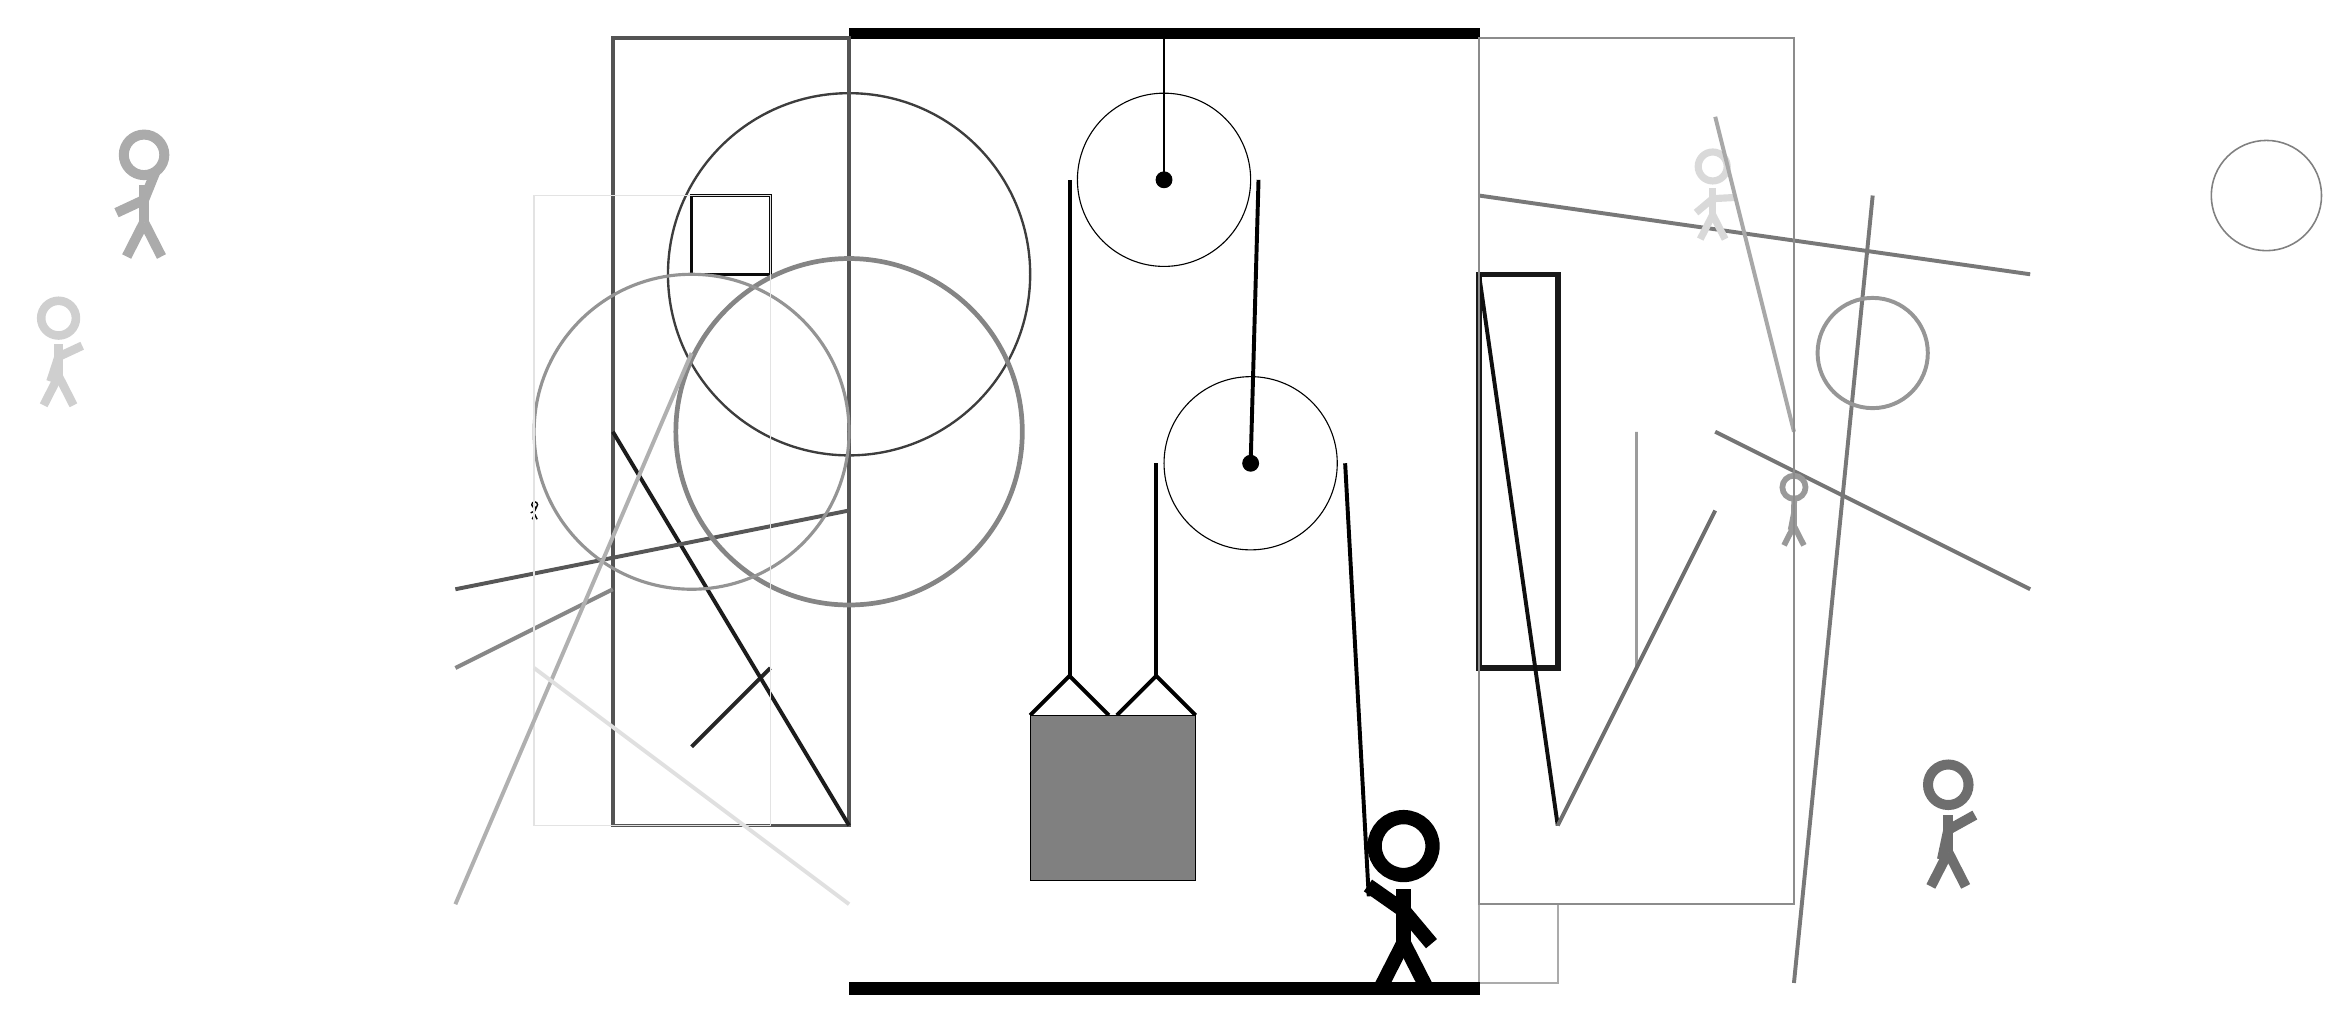
\begin{tikzpicture}
			%%%%% START %%%%%
			
			\draw[fill=black] (-2, 9) rectangle (6, 9.125);
			
			\draw (2, 7.2) circle (1.1);
			\draw[fill=black] (2, 7.2) circle (0.1);
			\draw[thick] (2, 7.2) -- (2, 9);
			
			\draw (3.1, 3.6) circle (1.1);
			\draw[fill=black] (3.1, 3.6) circle (0.1);
			
			\draw[line width=0.5mm, color=black!85](-4, 0) -- (-3, 1);
			
			\draw[line width=0.4mm, color=black!96] (-3, 7) rectangle (-4, 6);
			\draw[line width=0.2mm, color=black!33] (7, -2) rectangle (6, -3);
			\draw[line width=0.5mm, color=black!53](6, 7) -- (13, 6);
			\node[line width=0.5mm, color=black!15] at (9, 7) {\Strichmaxerl[5][40][3]};
			\draw[line width=0.5mm, color=black!34](9, 8) -- (10, 4);
			\draw[line width=0.5mm, color=black!54](9, 4) -- (13, 2);
			\draw [line width=0.3mm, color=black!76](-2, 6) circle (2.3);
			\draw[line width=0.5mm, color=black!67] (-2, -1) rectangle (-5, 9);
			\draw[line width=0.5mm, color=black!53](10, -3) -- (11, 7);
			
			\draw[line width=0.7mm, color=black!90] (6, 6) rectangle (7, 1);
			\draw[line width=0.5mm, color=black!47](-7, 1) -- (-5, 2);
			\draw[line width=0.5mm, color=black!39] (8, 4) rectangle (8, 1);
			\draw[line width=0.5mm, color=black!94](7, -1) -- (6, 6);
			\draw[line width=0.5mm, color=black!57](9, 3) -- (7, -1);
			\draw[line width=0.5mm, color=black!89](-2, -1) -- (-5, 4);
			\draw[line width=0.5mm, color=black!66](-2, 3) -- (-7, 2);
			\node[line width=0.6mm, color=black!98] at (-6, 3) {\Strichmaxerl[1][23][66]};
			\draw [line width=0.6mm, color=black!48](-2, 4) circle (2.2);
			
			\draw [line width=0.4mm, color=black!42](-4, 4) circle (2.0);
			\draw [line width=0.5mm, color=black!41](11, 5) circle (0.7);
			\node[line width=0.7mm, color=black!57] at (12, -1) {\Strichmaxerl[7][78][29]};
			
			\node[line width=0.6mm, color=black!40] at (10, 3) {\Strichmaxerl[4][79][89]};
			\draw[line width=0.2mm, color=black!11] (-3, -1) rectangle (-6, 7);
			\draw[line width=0.3mm, color=black!45] (6, -2) rectangle (10, 9);
			\node[line width=0.6mm, color=black!33] at (-11, 7) {\Strichmaxerl[7][25][68]};
			\draw[line width=0.5mm, color=black!31](-7, -2) -- (-4, 5);
			\node[line width=0.4mm, color=black!19] at (-12, 5) {\Strichmaxerl[6][72][25]};
			
			\draw [line width=0.2mm, color=black!50](16, 7) circle (0.7);
			\draw[line width=0.5mm, color=black!12](-2, -2) -- (-6, 1);
			
			\draw[line width = 0.5mm]  (0.3, 0.4) -- (0.8, 0.9) -- (1.3, 0.4);
			\draw[line width = 0.5mm]  (1.4, 0.4) -- (1.9, 0.9) -- (2.4, 0.4);
			\draw[fill=black!50] (0.3, 0.4) rectangle (2.4, -1.7);
			
			\draw[line width = 0.5mm] (0.8, 7.2) -- (0.8, 0.9);
			\centerarc[line width = 0.5mm](2, 7.2)(0:180:1.2000000000000002);
			\draw[line width = 0.5mm] (3.2, 7.2) -- (3.1, 3.6);
			\draw[line width = 0.5mm] (1.9, 3.6) -- (1.9, 0.9);
			\centerarc[line width = 0.5mm](3.1, 3.6)(0:180:1.2000000000000002);
			\draw[line width = 0.5mm] (4.3, 3.6) -- (4.6, -1.9);
			
			\node at (5, -2) {\Strichmaxerl[10][-35][-50]};
			
			\draw[fill=black] (-2, -3) rectangle (6, -3.15);
			
			%%%%% END %%%%%
		\end{tikzpicture}
	\end{figure}	
\end{document}